\documentclass[10pt, conference, compsocconf]{IEEEtran}
\usepackage{cite}
\usepackage{subfigure}
\ifCLASSINFOpdf
\usepackage[pdftex]{graphicx}
\graphicspath{{pdf/}{figures/}}
% and their extensions so you won’t have to specify these with
% every instance of \includegraphics
\DeclareGraphicsExtensions{.pdf,.jpeg,.png}
\else
% or other class option (dvipsone, dvipdf, if not using dvips). graphicx
% will default to the driver specified in the system graphics.cfg if no
% driver is specified.
\usepackage[dvips]{graphicx}
% declare the path(s) where your graphic files are
\graphicspath{{…/eps/}}
% and their extensions so you won’t have to specify fthese with
% every instance of \includegraphics
\DeclareGraphicsExtensions{.eps}
\fi

\usepackage{array}
\usepackage{multirow}
\usepackage{longtable}
\usepackage{rotating}
\usepackage[cmex10]{amsmath}
\usepackage{algorithmic}
\usepackage{array}
\usepackage{mdwmath}
\usepackage{mdwtab}
\usepackage{stfloats}
\usepackage{url}
\usepackage[colorlinks,
linkcolor=blue,
anchorcolor=blue,
citecolor=blue]{hyperref}
\hyphenation{op-tical net-works semi-conduc-tor}


\begin{document}
%
% paper title
% can use linebreaks \\ within to get better formatting as desired
\title{Docscanner: document location and enhancement based on image segmentation}

\author{\IEEEauthorblockN{Ziqi Shan\IEEEauthorrefmark{0},
% Xiaochun Lei$^{* 1,2}$\IEEEauthorrefmark{0}
Yuying Wang$^*$,\IEEEauthorrefmark{0}
Shunzhong Wei,\IEEEauthorrefmark{0}
Xiangmin Li,\IEEEauthorrefmark{0}
Haowen Pang\IEEEauthorrefmark{0}
and Xinmei Zhou\IEEEauthorrefmark{0}}
\IEEEauthorblockA{\IEEEauthorrefmark{0}School of computer and information security,\\
Guilin University of Electronic Technology,
Guilin 541004, China;}
% \IEEEauthorblockA{\IEEEauthorrefmark{0}2.Guangxi Key Laboratory of Image and Graphic Intelligent Processing, \\Guilin 541004, China;}
\IEEEauthorblockA{\IEEEauthorrefmark{1}Corresponding author's e-mail: getwyy@guet.edu.cn}}
% use for sepcial paper notices
%\IEEEspecialpapernotice{(Invited Paper)}
% make the title area
\maketitle
\begin{abstract}

Document scanning aims to transfer the captured photographs documents into scanned document files. 
However, current methods based on traditional or key point detection have the problem of low detection accuracy.
In this paper, we were the first to propose a document processing system based on semantic segmentation.
Our system uses OCRNet to segment documents.
Then, perspective transformation and other post-processing algorithms are used to obtain well-scanned documents based on the segmentation result.
Meanwhile, we optimized OCRNet's loss function and reached 97.25 MIoU on the test dataset.

\end{abstract}

\begin{IEEEkeywords}

Document Scanner, Document Processing, Semantic Segmentation.

\end{IEEEkeywords}

\IEEEpeerreviewmaketitle

\section{Introduction}

% introduce background

Document scanning systems have been widely used in many fields such as official business, administration, etc. 
With the demand for on-device document scanning increasing, document scanning systems are proposed to provide the office crowd with convenience. 

The current document scanning system is mainly based on traditional algorithms or keypoints detection.  \cite{Tropin2021AdvancedHM} proposed a advanced hough-based method for document localization. Javed et al.\cite{javed2017real} proposed a document keypoints detector based on cnn.
However, for most of those works, the quality of scanned images still can be improved to make a more accurate and robust document capturer.

We propose a document capturer based on semantic segmentation in this work and use advanced post-processing algorithms to gain well-scanned documents.
The system uses the OCRNet\cite{yuan2020object} to segment documents. 
OCRNet is based on the object-contextual representation scheme and can achieve a good document segmentation effect. According to the segmentation result, we can fit the four corners of the document. Then we use perspective transformation\cite{lin2010image} and other post-processing methods to make the well-scanned document.

\section{System Design}

\begin{figure}[!h]
\centering
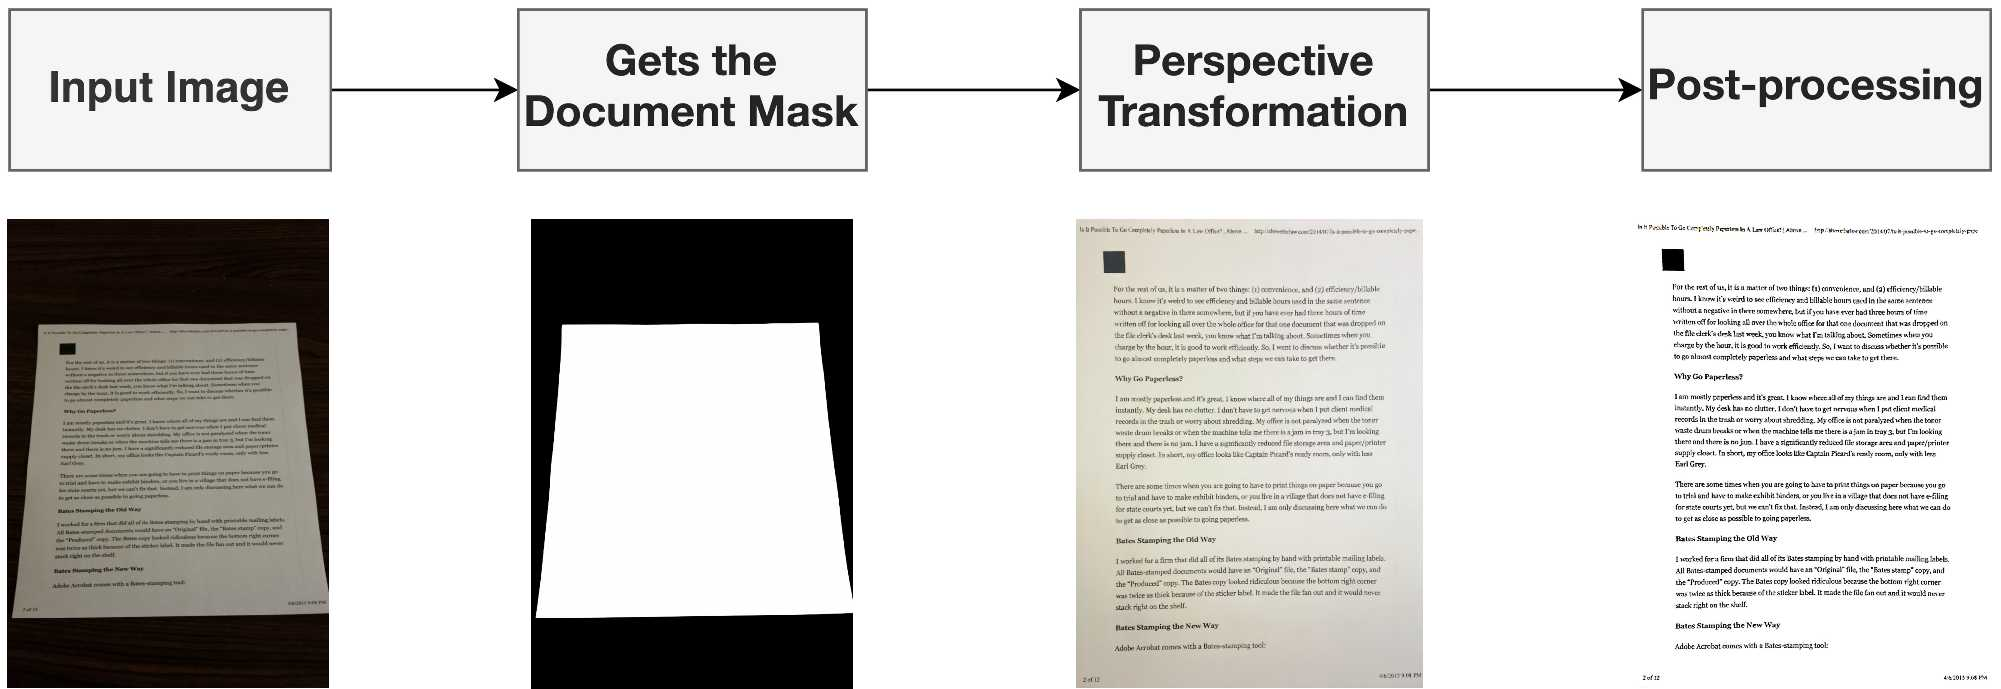
\includegraphics[width=3.2 in]{./Assets/FlowChart.jpg}
\caption{System Procedure}
\end{figure}


% give the statements.

Figure 1 shows the system procedure.
First, we use OCRNet\cite{yuan2020object} to get the document mask from the input image.
Second, we extract the four key points of the documents.
Then we apply a perspective transformation to convert the document image from a 3D image to a 2D scanned image.
Finally, we use binarization and other post-processing algorithms to enhance the document image. 

\section{Implementation}

\subsection{Image Segmentation}

Semantic segmentation has been widely used in many fields. 
We use OCRNet\cite{yuan2020object}, a semantic segmentation network, to segment documents in this system. 
OCRNet solves the context aggregation problem in semantic segmentation by using target regional representations to enhance its pixel representations, which improves the quality of segmentation results. 
We also use the Ohem cross-entropy\cite{shrivastava2016training} loss to solve the class imbalance problem. 

\subsubsection{Network Architecture}

\begin{figure*}[!h]
	\centering
	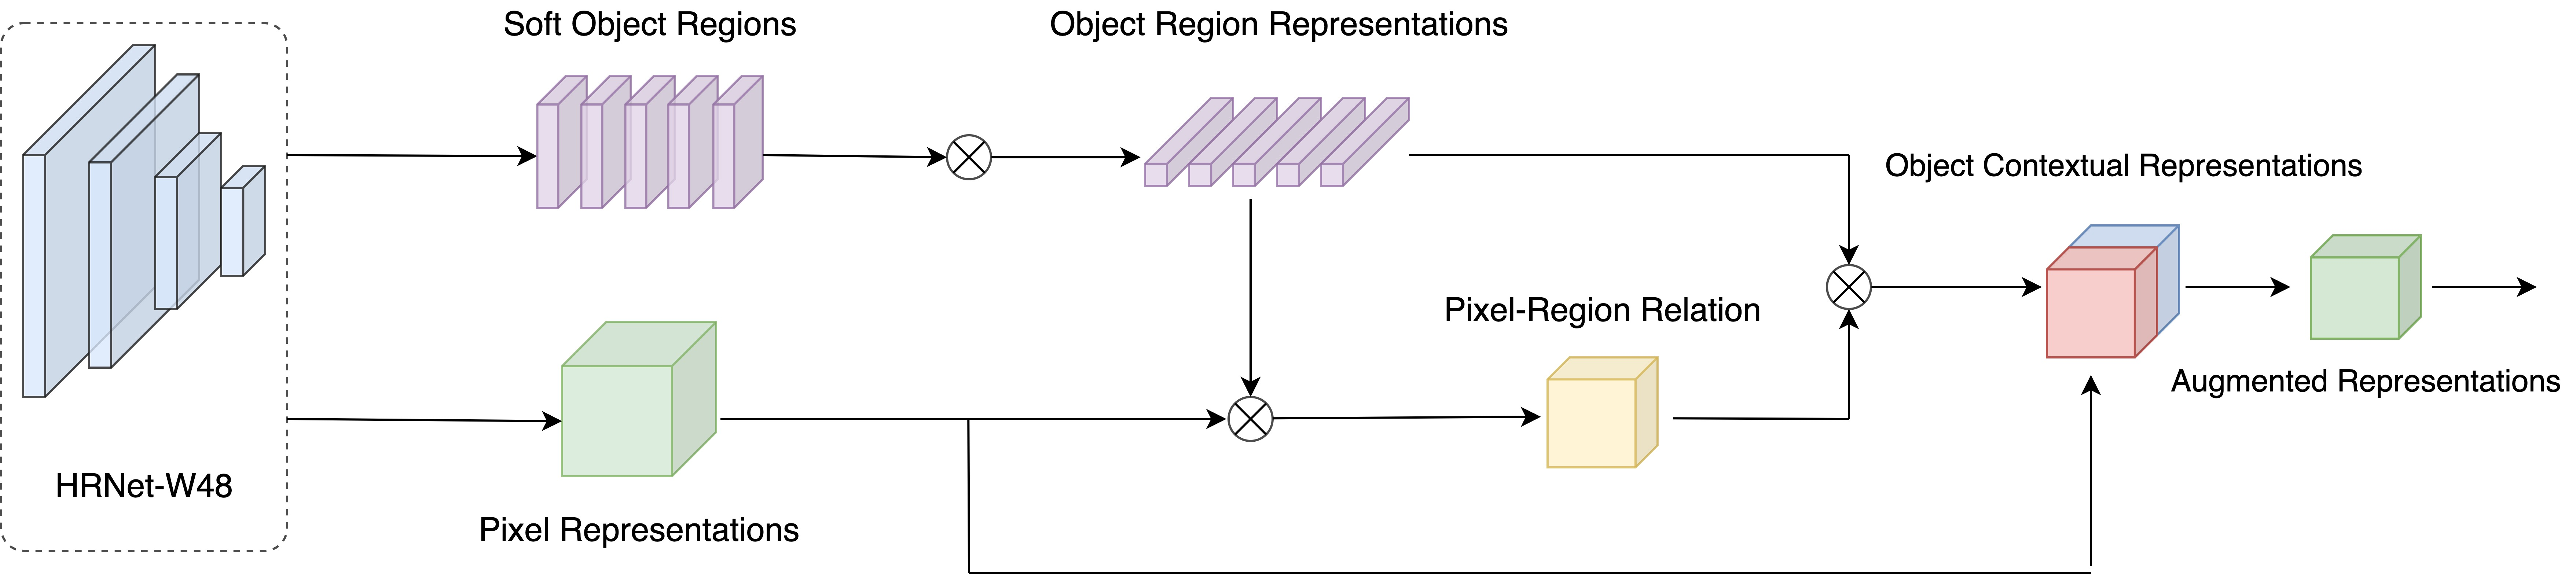
\includegraphics[width=7in]{./Assets/131245.jpg}
	\caption{The Architecture of OCRNet}
\end{figure*}

The architecture of OCRNet is shown in Figure 2. OCRNet in our system choose HRNet-W48\cite{wang2020deep} as the backbone. In the following stage, OCRNet first divides the contextual pixels into a set of soft object regions based on the output of the backbone. Each region corresponds to a class. Based on soft object regions and pixel representations of the backbone, OCRNet calculates a group vector called Object Region Representations. Each of these vectors corresponds to a semantic category's feature. Next, OCRNet will calculate the relations between pixel object regions. The OCR is the weighted aggregation of all the object region representations with the weights calculated according to the relations between pixels and object regions\cite{yuan2020object}. Finally, OCR and deep network features are combined as augmented representations.


\subsubsection{Loss Function}

The loss function of OCRNet in our system contains two parts: the Ohem cross-entropy loss\cite{shrivastava2016training} and the Dice loss\cite{milletari2016v}.
Ohem cross-entropy loss can help to solve the class imbalance problem. Dice loss is used to measure whether the predicted mask is close to the groundtruth. Our loss function is defined as follows:

\begin{equation}
	L = L_{Ohem} + w L_{Dice}
\end{equation}

$w$ is weight coefficient. We choose $w = 0.2$ in this work. $L_{Ohem}$ is the Ohem cross-entropy loss and $L_{Dice}$ is the Dice loss. Ohem cross-entropy loss, known as online hard example mining cross-entropy loss, is used to pay close attention to hard examples and set a higher weight. Let $\mathcal{M}$ be the predicted mask. $\mathcal{G}$ is the groundtruth mask of the image. $L_{Ohem}$ is defined as follows:

\begin{equation}
	L_{Ohem} = \sum_{i=1}^{N} \max_{i=1}^{N} \mathcal{M}_i log(\mathcal{G}_i) \\
\end{equation}

$L_{Ohem}$ first calculates each pixel's loss, then sums the top k loss items. It selects hard examples as training samples to improve the effect of network parameters. $L_{Dice}$ is derived from the dice coefficient and is often used as the metric function to estimate the comparability of two samples.  $L_{Dice}$ is defined as follows:

\begin{equation}
	L_{Dice} = 1 - \frac{2|\mathcal{M} \cap \mathcal{G}|}{|\mathcal{M}| + |\mathcal{G}|}
\end{equation}


\subsection{Perspective Transformation}

% fitting the keyt points
% https://blog.csdn.net/ooooocj/article/details/110936343
After we obtain the predicted mask, we can carry the perspective transformation to the image according to the mask.
The process is shown in the Figure 3. First, we use the canny\cite{bao2005canny} algorithm to extract the edge of the mask. Then we use the Douglas-Peucker algorithm\cite{wu2004douglas} to find the four corners of the edge. According to the key points, we can calculate the perspective transformation matrix. Then we apply the perspective transformation to the image according to the matrix to convert it from a 3D image to a 2D image.


\begin{figure}[!h]
	\centering
	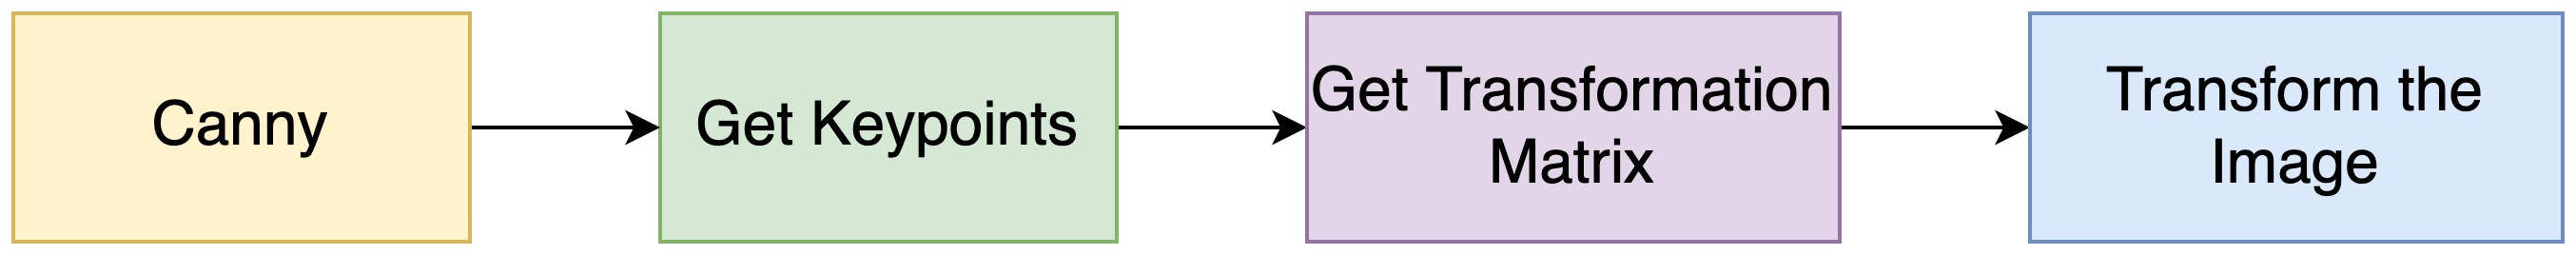
\includegraphics[width=2.8in]{./Assets/123.jpg}
	\caption{The process of perspective transformation}
\end{figure}

\subsection{Post Processing}

\label{post-process}

% why use it : make image clear & keep colorful (maybe need to mention the low space usage).
At the last step, we obtain the 2D view document image. In order to get the better quality of the document image, we use post-processing algorithms to enhance the document image. The post-processing algorithms mainly include separating the background and foreground colours.

\subsubsection{Separate Background Colors}

% recognize background color of raw scanned images
The usual method to separate background colours is by analyzing the number of pixel values.
However, even the largest number pixel value of an 8-bit colour image is a tiny percentage (under 10\%) of all pixels.
Therefore, we convert an 8-bit channel colour image to a 6-bit channel colour image.
Reducing the pixel type will help determine the background colour.
By analyzing the 6-bit colour image's pixel value number, we can determine the background colour. Document images are enhanced by replacing the background colour with white.

\subsubsection{Separate Foreground Colors}

\label{separate-foreground-colors}
Once the background colour has been identified, we can calculate the foreground colour by calculating how similar each pixel is to the background colour.
We first convert the image to HSV color space.
Then we calculate the European distance between each pixel and the background colour.
To make the image more colourful, we cluster the foreground pixels into eight groups using k-means\cite{hartigan1979algorithm}. 
We will assign every foreground colour to one of the eight groups. 


\section{Experiments}

This section will introduce the experiment setup, image segmentation, and post-processing result. We will also compare different image segmentation methods and post-processing methods. 
% the experiment software & hardware environment

\begin{table}
	\caption{Experiment Environment}
	\begin{tabular}{cc}
		\hline Equipment & Configuration Information \\
		\hline CPU & Intel(R) Xeon(R) Gold CPU @ 3.00GHz \\
		 RAM & 64G \\
		 GPU & Tesla V100-PCIE-32GB \\
		 OS & Ubuntu 16.04.3 LTS \\
		 Programming Language & Python \\
		 DL Framework & PaddlePaddle \\
		\hline
	\end{tabular}
\end{table}

\subsection{Experiment Setup}


Our experiment environment is shown in Table 1. 
We use Baidu open source dataset containing 3,000 images. 
We choose the OCRNet\cite{yuan2020object} and U-net\cite{ronneberger2015u} for image segmentation to compare the result.
For the post-processing algorithm, we compare the adaptive binarization method and our method described in Section \ref{post-process}.
For our experiments, we use Baidu's open-source document dataset. 




\subsection{Experiment Results}

\begin{figure}[!t]
	\centering
	\label{figure:Comparition}
	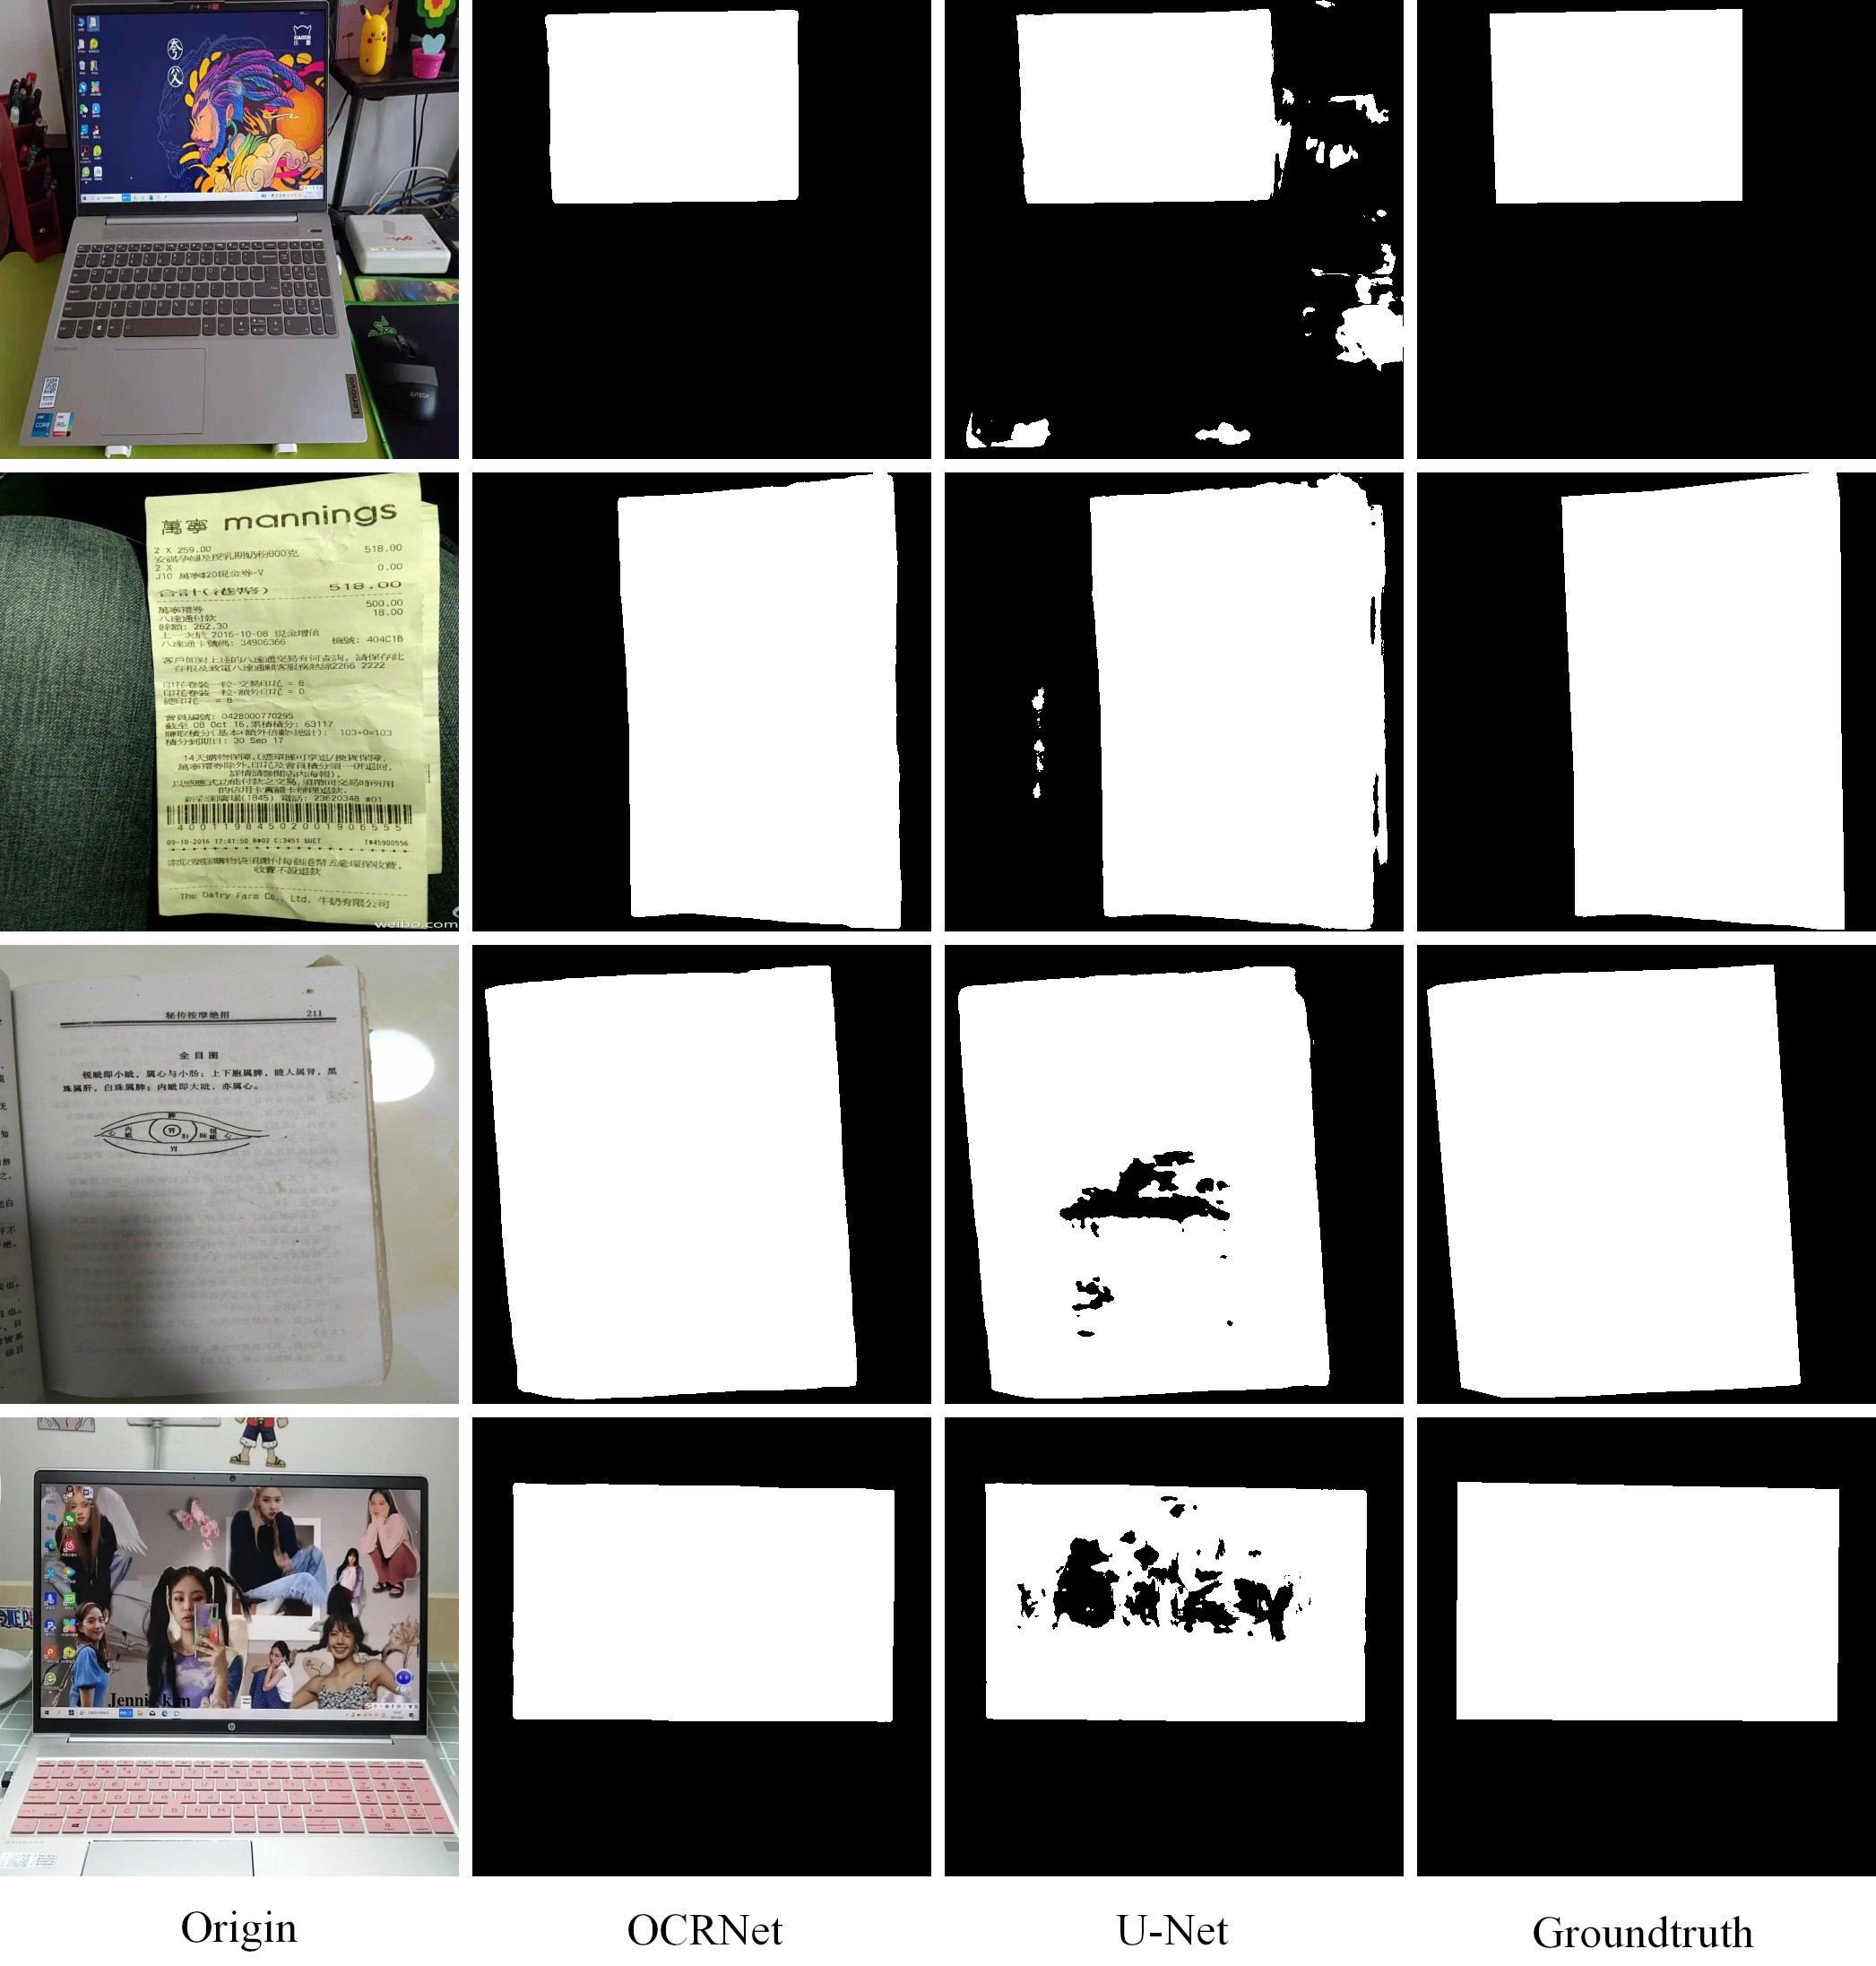
\includegraphics[width=3.2in]{./Assets/final_whole_img.jpg}
	\caption{Comparition between OCRNet and UNet}
\end{figure}
	

\subsubsection{Image Segmentation}

We compare three groups of image segmentation methods: OCRNet(without the Ohem loss), U-Net, and OCRNet(Ours). 
The experiment result is shown in Table \ref{table:comparition}.
OCRNet(Ours) achieve the best result (94.14\% miou) on the test dataset.
By comparing OCRNet with U-Net, we can find that U-Net's prediction masks have some holes, as shown in Figure \ref{figure:Comparition}. 
OCRNet, because of its context aggregation strategy, performs excellently in document segmentation.

\begin{table}[!h]
	\caption{The Comparison of Different Models}
	\centering
	\label{table:comparition}
	\begin{tabular}{ccc} \\
	\hline
	Model & MIoU(\%) & Mean Acc(\%)\\
	\hline
	OCRNet(Origin) & 94.14 & 96.15\\
	U-Net & 94.46 & 96.64\\
	OCRNet(Ours) & 97.26 & 99.36\\
	\hline
	\end{tabular}
\end{table}

\subsubsection{Image Post Processing}
% the used dataset
We compare two image post processing method: adaptive binarization and our method. 
Adaptive binarization is widely used in image enhancement. 
Our method is based on the idea of separation of foreground and background and is described at Section \ref{separate-foreground-colors}.
Figure \ref{figure:post-process} show the comparition of the two methods.
Adaptive binarization performs better when the image is not noisy.
However, when the image is noisy, the adaptive binarization method is unsuitable, as shown in the third row of Figure \ref{figure:post-process}.
In the meantime, adaptive binarization will result in grayscale images.
Our method is better when the image is noisy. 
And we can make the scanned document colorful.

\begin{figure}[!h]
	\centering
	\label{figure:post-process}
	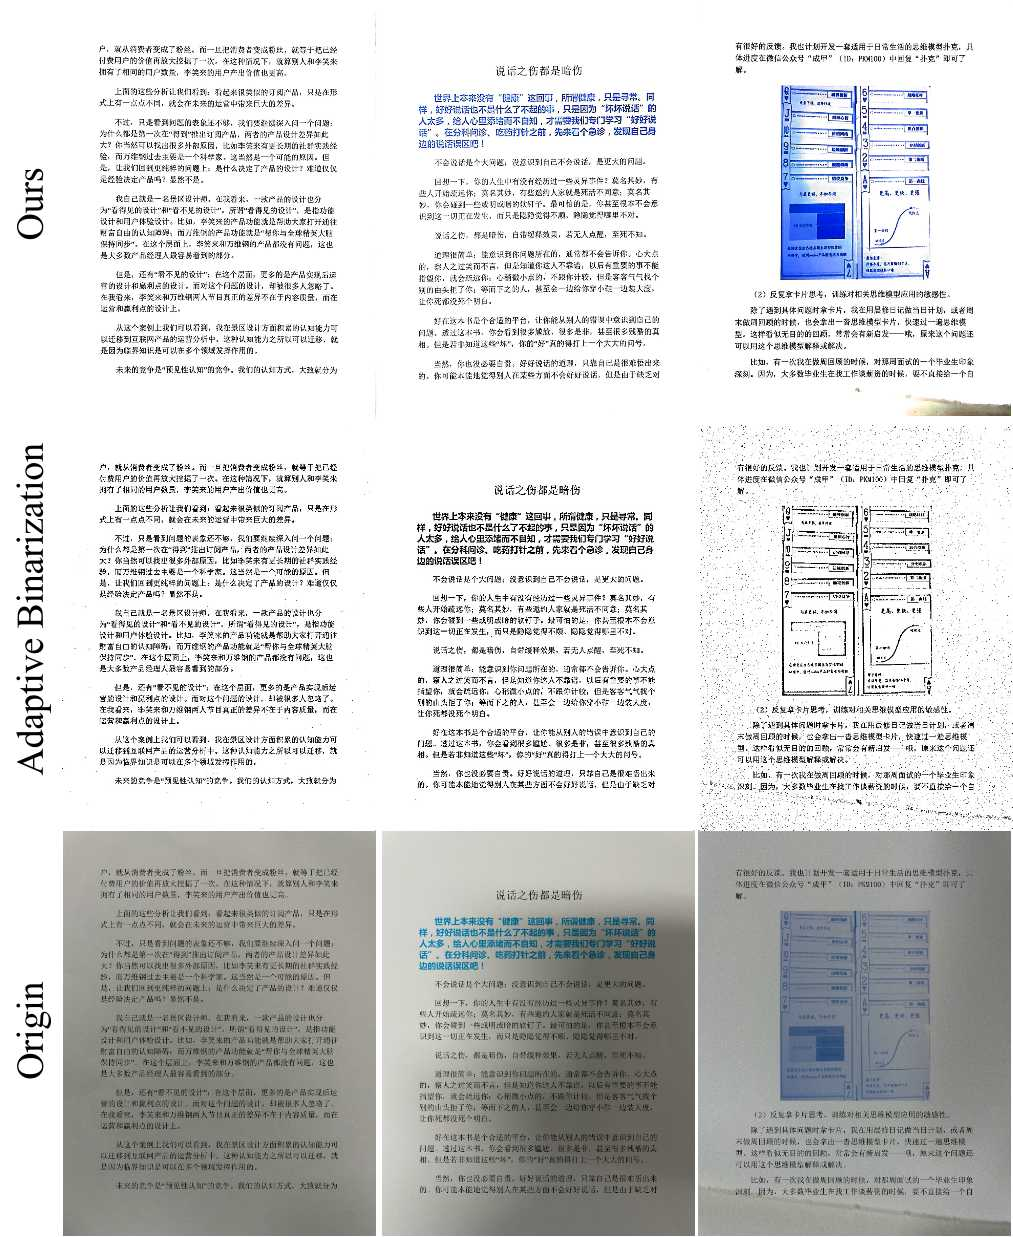
\includegraphics[width=3.0in]{./Assets/12345.jpg}
	\caption{Post-processing Method Comparition}
\end{figure}



\section{Conclusion}

In this paper, we build a document scanning system to generate precise and colorful results.
The system is based on image segmentation. We use OCRNet to produce the document segmentation mask. Meanwhile, we use a mixed loss function combining Ohem cross entropy and dice loss to improve the model.
We also use an advanced post-processing method to enhance the scanned image.



% use section* for acknowledgement
\section*{Acknowledgment}

This work is supported by Student’s Platform for Innovation and Entrepreneurship Training Program under Grant (202110595025).

%This essay is supported by Project to Improve the scientific research basic ability of Middle-aged and Young Teachers (No.2019ky0222,2020KY05033),the Open Funds Guangxi Key Laboratory of Image and Graphic Intelligent Processing, No.GIIP2004, Student's Platform for Innovation and Entrepreneurship Training Program under Grant (No.202010595053. 202010595022)

% trigger a \newpage just before the given reference
% number - used to balance the columns on the last page
% adjust value as needed - may need to be readjusted if
% the document is modified later
%\IEEEtriggeratref{8}
% The "triggered" command can be changed if desired:
%\IEEEtriggercmd{\enlargethispage{-5in}}

% references section

% can use a bibliography generated by BibTeX as a .bbl file
% BibTeX documentation can be easily obtained at:
% http://www.ctan.org/tex-archive/biblio/bibtex/contrib/doc/
% The IEEEtran BibTeX style support page is at:
% http://www.michaelshell.org/tex/ieeetran/bibtex/
%\bibliographystyle{IEEEtran}
% argument is your BibTeX string definitions and bibliography database(s)
%\bibliography{IEEEabrv,../bib/paper}
%
% <OR> manually copy in the resultant .bbl file
% set second argument of \begin to the number of references
% (used to reserve space for the reference number labels box)

% 导入bib
\bibliographystyle{IEEEtran}
\bibliography{Document-Scanner-EI-Paper}


\end{document}
